\section{Application}
\label{Application}
	\subsection{Information Procurement}
	The main theme of the collected data would concentrate around the topic of Internet sales platforms also known as E-Commerce. Several aspects make the topic beneficial for this research. Firstly, the very nature of E-Commerce. By nature of E-Commerce Platforms, I refer to the fact, that such companies are almost exclusively web-based. It is therefore probable that most of the company's marketing efforts as well as overall news relating to such a company, would circulate first and foremost in the Internet. Secondly, having all company-relevant news attainable foremost from the web, means that such news would seep to social media faster in comparison to news, which are usually covered initially by traditional media such as television and Newspapers. 
	
		\subsubsection*{Search Terms}
		The data was collected in the form of relevant Tweets from the Twitter Stream API. A Tweet would be considered relevant if it contained a search parameter related contextually to E-Commerce. The initial efforts were concentrated around the web-store Amazon. Amazon appears to the most fruitful search parameter in terms of the quantity of Tweets relating to it. Additional search words that were tested were {\bfseries Alibaba, Zalando} and {\bfseries Groupon}. 
		The widespread mention of Amazon in Tweets is however somewhat over-inflated due to the extensive use of Amazon gift cards. Amazon gift-cards have become prominent due their variety of uses. A few examples of common practices involving Amazon gift cards are rewarding users for services, such as polls and questionnaires, enticing people to take part in events or groups, and being offered as general rewards in competitions and games. The plethora of uses, facilitates Amazon gift cards to be viewed as a sort of pseudo-currency in the Internet. In turn this means, that Amazon could be mentioned in a Tweet, despite the context only indicating the Gift-card and being completely unassociated to the E-Commerce platform whatsoever.
		
		\subsubsection*{Collecting the Data}
		\label{sec:collect_data}
		The gathering of Tweets was executed using a program written by me in the Python programming language. The main module being used in the program was a Twitter Streaming API called Tweepy. Tweepy is an open source interface, which allows communicating with the Twitters servers and sending queries requesting specific information from Twitter's databases. The interface allows for two main type of queries, Rest and Streaming. The former allows looking up information posted on Twitter in the past whereas the latter, as the name implies connects to an active data stream containing a narrowed down flow of Tweets being actively published by Twitter users. Both types of API's are being offered for free to a certain extent, whereas almost unrestricted versions of the same API are offered as a proprietary fee-based product of Twitter. The free version of the REST API is restricted to only looking up Tweets posted in the last two to three weeks. And the gratis version of the Streaming API is restricted to a fire-hose narrowed down to about 15\% of the total Bandwidth of all current Tweets.
		The Tweets from the Twitter servers come in form of JSON strings, which allows for embedding other JSON objects in them, which allows for multi-level storage of Tweet properties. For example, one of the JSON objects integrated in each Tweet JSON object is the USER object for the Tweet-poster. The USER object in turn contains all data publicly available in Twitter about a Twitter account such as, location, date of registration, homepage etc. An additional object of interest is the ENTITIES JSON object, which contains all outside references from the Tweet's text such as, URLs, Multimedia, References to other Tweets or other users. 
		This structure greatly eases the construction an analysis of a Tweet and its features, since most of the necessary data is available from the Tweet self and no further queries about the Tweets and its posting-user are necessary.
		\par
		{\LARGE \color{red}
			elaborate about stages of data collection:
		} \\ 
		{\color{red}
			1. Initial data: full of duplicates\\
			2. Filtered data - fewer duplicates and Spam, but still rather very one-subject-centered. Leads to overfitting when classifying \\
			3. still untried - collect up to x (~400) Tweets per day, for a duration of ~ 2 weeks
		}
		
		\subsubsection*{Data cleansing}
		It was observed that numerous Tweets were being posted more than once and in several occurrences even hundreds of times. These duplicates were being primarily posted by bots, as was evident from a short observation of user profiles belonging the Tweets original posters. Evidently, additional effort was being made by the programmers of the bots to try and mask them by slightly altering the content of the Tweets, or the user account. This was usually done by changing or adding characters to the text, which carry no lingual significance in themselves. Moreover, in furtherance of increasing the bots' credibility as an actual people \hyperref[fig:twitterbot]{(Fig. 1)}, often times entire nets of such bot could be observed, wherein the bots would maintain friendship and following connections among themselves. This in turn, further adding to each of them having a multiplicity of friends and followers contributing to their veil of disguise as real human users of Tweeter. Upon closer observation such accounts reveal their true essence, since most of the content propagated by them is commercial in nature and is repeated verbatim time and again across many of the related accounts \textit{followers} and \textit{friends}, it would be safe to assume that no actual people are behind them. 
		\par
		
		\begin{figure}[h]
			\centering
			\label{fig:twitterbot}
			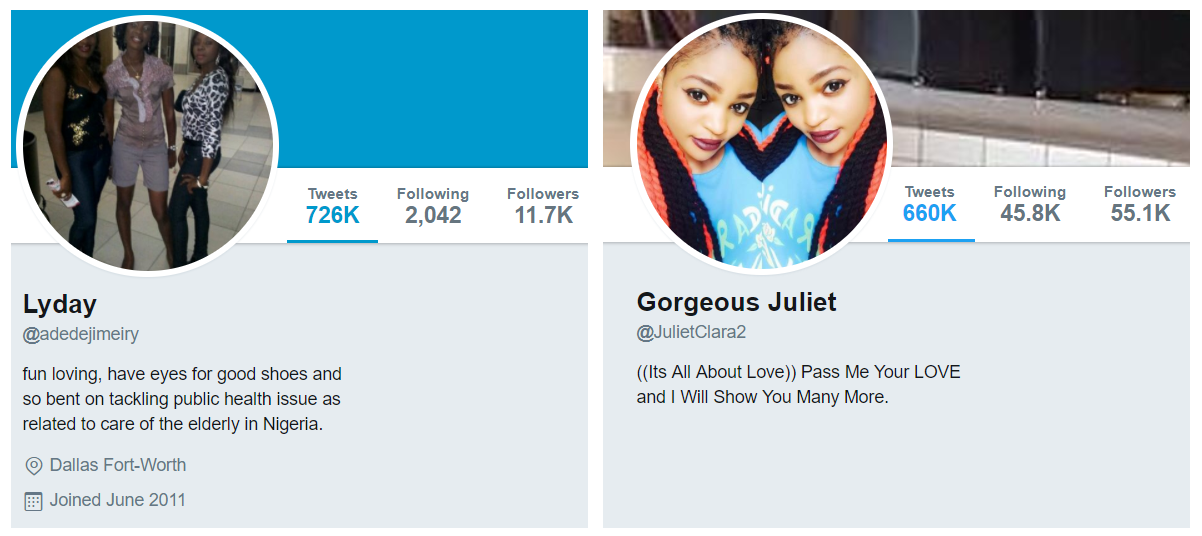
\includegraphics[width=0.5\textwidth]{twitterbot.PNG}
			\caption{Twitter accounts, which present themselves as actual people}
		\end{figure}
		
		\newpage
		\noindent
		Several precautions were undertaken to try and filter out such bots. A passive precaution which was implemented, was blacklisting users, which had priorly been observed posting Tweets, which were verbatim copies of other Tweets within the same query. The suspected users were added to a suspect database and content originating from them was ignored in future queries. Another action made with the same purpose in mind was a retrospective cleanup of the collected Tweets, based on their content similarity. After closing a collection query, a maximum similarity measure for each Tweet in relation to all other recorded Tweets was calculated using a simple . Following, Tweets which were found to have a maximal similarity score to other previously captured Tweets  higher than a predetermined threshold were classified as non-unique copies and were disregarded. As a measure of similarity, the S\o rensen-Dice coefficient\cite{sorensen1948method} \hyperref[fig:sorenson_dice]{(Fig. 2)} was implemented using the \textit{SequenceMatcher.ratio()} function from the difflib Python module {\color{red} \Large also try Levenshtein }. A round of cleanup using this procedure would usually reduce a data set by from one quarter and up to one half of its original size.
		
		\begin{figure}[h]
			\begin{center}
				\label{fig:sorenson_dice}
				$QS_{XY} = \dfrac{2|X\cap Y|}{|X|+|Y|},$ \hspace{10pt}  $QS_{XY} \in [0:1]$
				\par
			\end{center}
			{\small
				* $|X|$ and $|Y|$ are the numbers of elements in given Tweets X and Y accordingly 
				\\
				** QS ranges from 0 (completely different) to 1 (identical)
				\caption{S\o rensen-Dice coefficient}
			}
		\end{figure}
		
		\newpage
		
	\subsection{Building the Datasets}
	\label{build_features}
	Once a list of labeled Tweets is obtained, the next stage is constructing a feature-set to be later passed on as input for training an ML Classifier. The features contained if the feature sets describe certain aspects and characteristics of a Tweet and its owner. Two main approaches to feature sets are found in the literature, \textit{Word-Based} also often called \textit{Bag-of-Words} as can be observed in \textbf{\color{red} insert citation} and \textit{Descriptive} \textbf{\color{red} insert citation}. 
	
		\subsubsection{Word-Based Features}
		The former approach simply converts the entire text corpus to a frequency charts of all the words contained within. Words are then selected to act as features in incoming data, which is to be classified. The features are hence a variable list (usually of several thousands in length), where each variable is a boolean representation, indicating the presence or absence of a certain word. Usually the words undergo preprocessing as is common in Natural Language Processing prior to being used as features. The corpora are segmented to lists of words, often omitting articles, proposition and punctuation. Such grammatical structures are critical in human speech and writing ind order to convey ones meaning clearly and explicitly, however for the purposes of more ambiguous classification as in our case, such nuances are avoided for the sake of simplicity. Words are then \textit{stemmed} or \textit{lemmatized}, meaning their are reverted to their grammatical stem - dropping all prefixes and suffixes. This eases the enumeration of words, since it is preferable that the same words in different inclinations would be counted as the same. For example, the word pair \textit{eating} and \textit{ate} would be reverted to their stem \textit{eat}, as well as \textit{apple} and \textit{apples} would be considered as one and the same. Finally, words would be assigned their part of speech (noun, verb, adjective ..) and could be either ignored or incorporated into the feature set, according to the conceived importance of a given part of speech.
		
		
		\subsubsection{Descriptive Features}
		The latter approach mentioned is based of more generalized view of the Tweet, instead of concentrating on the actual textual content. Descriptive features are aimed at describing the Tweet implicit properties, such as attitude, sentiment, seriousness and trustworthiness. These features detect presence of different symbols, their frequency and consecutiveness. Additionally, unlike the Web-Based approach, non-textual objects such as multimedia, links and mentions of other users and Tweets are also taken into account. Furthermore, features of a Tweets owner are included alongside. Since Tweeters API provides a complete user profile incorporated inside the Tweet data object itself, constructing features describing the user is done simultaneously to features describing the content of the Tweet itself. This approach might be viewed as an \textit{indirect} one, since less obvious properties of the Tweet are used to characterize it.
		\par
		Descriptive features could be segregated into three distinctive groups. The first will be referred to as text-based features. As the name suggests, the features will mostly denote the presence or lack of specific characters such as emoticons and signs in the Tweets text. Whether a Tweet contains combinations or sequences of certain symbols as well as ratios defining the text also befit this category.
		\par
		The second tier of features describe any special \textit{Entities} (Tweeter's nomenclature) contained within a Tweet. \textit{Entities} refer to non-textual contents of a Tweet such as media (in form of pictures, sound or videos), URL's linking to external websites, Mentions or ReTweets (Referring to other Tweets or to Tweeter user profiles) and finally Hashtags. A word or phrase preceded by the Hashtag symbol \textbf{\#} indicate the association of web content (such as a Tweet or other micro-blogging post) to a specific theme such as an event, news, gossip or any other tidbit \cite{dict_Tweet}. Hashtags are used primarily to simplify looking up Tweets or other social media content by technically associating them with the \textit{hashtagged} topic.
		\par
		{\color{red}The third tier - subject}
		
		
	\subsection{Training Classifier}
	The purpose of \textit{training} is to create Classifiers, which automatically recognize and \textit{label} new observations. The intrinsic	decision algorithm, through which the Classifier will decide how to classify a novel observation, usually remain hidden and operate as a black-box of sorts. Since the decision rules could be numerous and far from intuitive for human readers. This is especially the case, when said algorithms are convolutional. Convolutional machine learning schemes, such as Deep Neural Networks, may incorporate numerous stages of parameter construction which renders them practically incomprehensible to human users. The actual implementation of all the algorithms would be programmed in the Python programming language and will be primarily making use of the scikit-learn\cite{scikit-learn} module.
	\par
	The data used for the purpose of this study consolidates 12.520 unique Tweets. For the purpose of reaching robust results, the \textit{Hold-out Method} is used as follows. For each instance of \textit{Algorithm training} the entire data corpus is split into two parts - a training set and testing set. The training set would usually be allocated the larger portion of the data (about 70\%) and would be used, as the name suggests for training the Classifiers. The rest of the data (about 30\%) would be used for testing the Classifiers accuracy. During each such training-testing session, the data corpus is shuffled. This in turn means, that the training and testing sets constantly differ. This process of splitting, training and testing using different data in each iteration should produce statistically significant results. This method of constantly splitting the data randomly ensures the results robustness.
	\par
	The following paragraphs expand on the different Machine Learning schemes. Figure 3 illustrates these schemes according to their types.
	
	\begin{figure}[h]
		
		\centering
		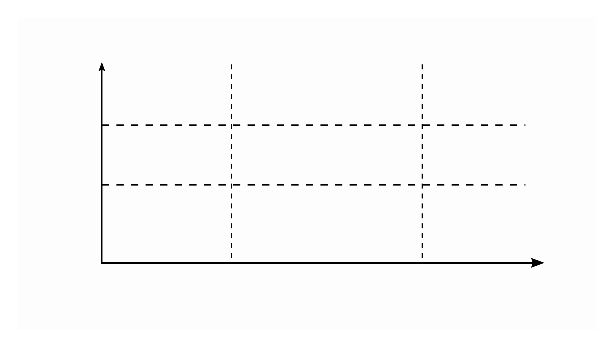
\includegraphics[width=0.5\textwidth]{methods}
		\caption{Clustering of Different Classifiers}
	\end{figure}

	\subsection{Classifier Types}
	
		\subsubsection*{Regressions}
		One approach and probably the most basic one is simply running a regression with all the features as the independent variables and the a numeric representation of the classes as the dependent variable. Some threshold value for the classes must be determined since the estimate for the explained variable, will have a non-deterministic value.
		\par
			\paragraph{Linear Regression} 
			This method builds a linear dependency system between the explained variable (the \textit{Class} in this case) and the explaining variables (\textit{features}). With the \textit{Bag-of-Words} approach, each variable \textit{x} is a dummy variable indicating whether a given word \textit{m} is present in Tweet \textit{i}. The estimations parameters, which are denoted with $\beta_j$ are derived using Ordinary Least Squares. In itself, the linear regression estimation is a weak predictor for the purpose of classification, but it allows for calculating other useful statistics such as the coefficient of determination, commonly known as $R^2$. This static demonstrates the part of the variance that is explained using the provided variables and is also sometimes called 'goodness of fit'. We therefore strive to maximize it as much as possible. The more of the variance that is covered by our variables, the better can we predict the out come of the classification. Another point of interest is the distribution of predicted classifications ($\hat{y}$). In an ideal scenario, the distribution of $\hat{y}$ would be concentrated around the numerical representations of the two classed, as follows:
			
			\begin{equation}
				\mathbb{E}(\hat{y} \ \vert \ label) \approx \begin{cases}
				1,   & \text{for } label = \text{News}\\
				2, & \text{for } label = \text{Not News}
				\end{cases}
			\end{equation}
			
			\newpage
			
			\hyperref[Linear_Regression]{Equation 2} shows the basic scheme for the use of linear regressions as classification tools, where n is the number of observations, m is the number of features.
			
			\begin{equation}
				y_i = \beta_1 x_{1i}+ \beta_2 x_{2i} + ... + \beta_m x_{mi} + \epsilon_i \ \ \ \ \ \ \ \ 
				\forall \ i \in [1,n].
				\label{Linear_Regression}
			\end{equation}
			
			\paragraph{Logistic Regression} This regression scheme differs from linear firstly, in the fact, that the possible outcomes of the dependent variable are discreet rather than continuous. This allows for a much more fluent application as a classification tool and is therefore commonly employed in  Machine Learning. Logistic regression analysis is formally represented as follows in  \hyperref[logit]{Equation 3}
			
			\begin{equation}
				y = 
				\begin{cases}
				1 \ \  \beta_0 + \beta_1 x + \epsilon > 0 \\
				0 \ \  \text{else } 
				\end{cases} \text{         } \forall \  x = 
				\begin{pmatrix}x_1\\x_2\\...\\x_n \end{pmatrix}
			\end{equation}
			
			The $x$ vector represents all explanatory variables, in our case, the Tweet features. The term error $\epsilon$ is distributed by the standard logistic distribution, which also gives the regression its name.
	
	
	
	
		
		
		
		